\chapter{Networking}
\label{ch:networking}

\author{Nico Kratky}
%
\section{Networking in GRAMOC}

Because GRAMOC is based on basic a client-server architecture, a common way of communication had to be developed. This development process resulted in GSDEP, which stands for \textbf{G}RAMOC \textbf{S}ensor \textbf{D}ata \textbf{E}xchange \textbf{P}rotocol.

As sensor data is received over the internet and it should also be delivered to clients wirelessly, a common way of communication had to be developed. This development process resulted in GSDEP, GRAMOC's networking protocol. It is a TCP-based networking protocol that is used for sending large amounts of sensor data \cite{rfc793}.

\section{Data Flow}
\label{sec:networking_data-flow}

Figure \vref{fig:handshake} depicts the handshake performed by GSDEP that is based on TCP's three-way handshake. The client sends a synchronize (SYN) message to the server to let it know that it wants to connect. If the server can accept new Clients it returns an acknowledgment message (ACK). The client then also returns this acknowledgment message to inform the server that it is indeed connected. The connection now is established and data can be transmitted.

\begin{figure}[h]
    \centering
    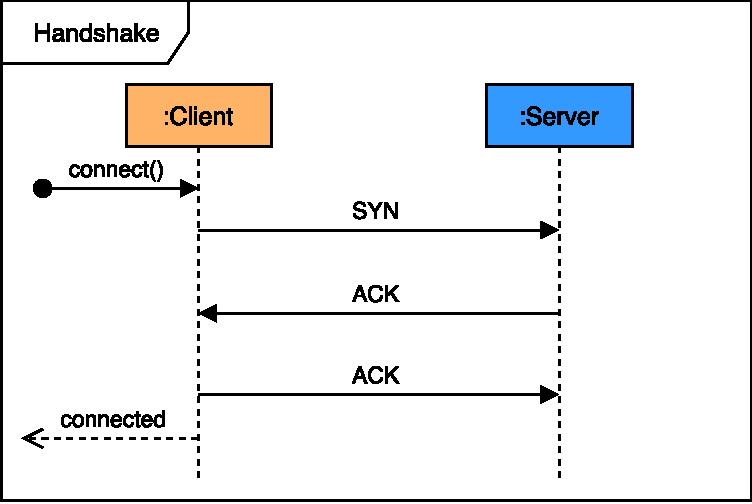
\includegraphics[width=8cm,keepaspectratio]{gsdep_handshake}
    \caption{TCP-like three way handshake performed on client connect}
    \label{fig:handshake}
\end{figure}

If a client wants to disconnect from the server it will send a disconnect message (FIN) to the server. Before it actually disconnects, it has to wait for the server to finish cleaning up and return the FIN packet. After the client has received this message, it can close the connection and shut down. This procedure is shown in figure \vref{fig:disconnect}.

\begin{figure}[h]
    \centering
    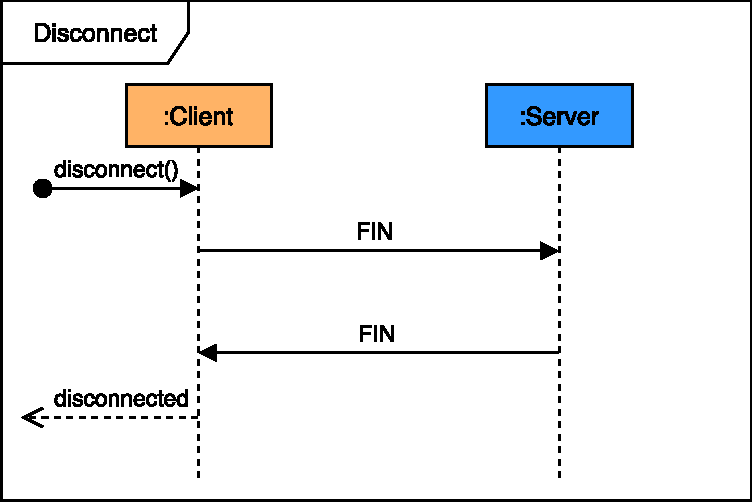
\includegraphics[width=8cm,keepaspectratio]{gsdep_disconnect}
    \caption{Two way handshake performed on client disconnect}
    \label{fig:disconnect}
\end{figure}

\section{Data Interchange Format}

Message have to be brought to a common format to be understood be all communication partners. Therefore every message transmitted is prefixed with a header. This header includes additional information that is used by the receiving end to determine the size of the payload (see \vref{sec:messageframing}), to differentiate between different kinds of messages (see \vref{sec:channels}) and to rebuild the message data to its correct data type. The header consists of of 8 bytes, 4 are used to store the payload length, and 2 bytes each for data type and channel. A example packet is illustrated in figure \vref{fig:packet}.

\begin{figure}[h]
    \centering
    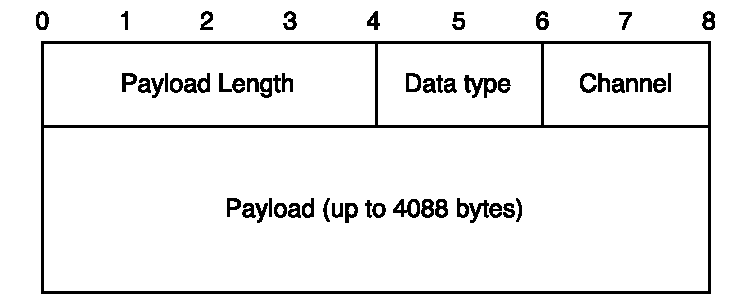
\includegraphics[width=8cm,keepaspectratio]{gsdep_packet}
    \caption{Structure and field sizes of a packed message sent with GSDEP}
    \label{fig:packet}
\end{figure}

\section{Commands}
\label{sec:networking_command}

Commands are special message that are used to prompt the other end to do something. These commands are used for two purposes. On the one hand they are used during the connection establishment and termination phases, and on the other hand they are used to request data or to stop data transmission.

\begin{table}[h]
    \centering
    \begin{tabular}{| l | l | p{5cm} |}
    \hline
    \textbf{Command} & \textbf{Used by} & \textbf{Meaning} \\ \hline
    SYN & client & Tells the server that a new client is waiting for the connection procedure \\ \hline
    ACK & server \& client & Tells the other end that it acknowledges the previous command \\ \hline
    FIN & server \& client & Tells the other end that it will disconnect \\ \hline
    STD & client & Tells the server that a client requests data\\ \hline
    SPD & client & Tells the server that a client does not want any more data\\
    \hline
    \end{tabular}
    \caption{Commands sent by one of the connection partners and what they do}
    \label{tab:commands}
\end{table}

\section{Channels}
\label{sec:channels}

In the case of GRAMOC, where large amounts of data are received in short periods of time, it is crucial to differentiate between communication data and sensor data in split seconds. To accomplish this, 2 bytes are included in the message header. This field simply contains numbers that represent different channels (figure \vref{tab:channels} shows these channels). This information can then be used by the client to tell apart these two types of data, without even analyzing the payload.

\begin{table}[h]
    \centering
    \begin{tabular}{| l | c |}
    \hline
    \textbf{Channel} & \textbf{Value} \\ \hline
    Communication & 1 \\ \hline
    Data & 2 \\
    \hline
    \end{tabular}
    \caption{Channels used to distinguish between message types}
    \label{tab:channels}
\end{table}

\section{Message framing}
\label{sec:messageframing}

A common mistake that many developers make is to assume that TCP operates with messages and that TCP can tell apart these messages \cite{MessageFramingCleary,MessageFramingSkotzko}. Sadly this is not true as TCP operates with continous streams of data. Therefore the differentiation of messages has to be done by the developers. This can be achieved in two ways.

\subsection{Delimiters}

\subsubsection{Sending}

Using delimiters probably is the simplest solution. This can be done by sending a special character between each message. This character can either be a character that does not show up in actual messages (e.g. a Null character), or a character that is present in a message. If the second approach is used, every message has to be run through an escaping process which replaces these characters in the messages.

\subsubsection{Receiving}

Receiving delimited messages is relatively straightforward. The program knows that a message has been fully read when it encounters a delimiter character. This message then has to be passed to an unescaping function when a delimiter character is chosen that can exist in messages.

\subsection{Length Prefixing}

Another method of message framing is to prefix each message with its length. When doing so the format of this prefix has to be stated explicitly. In the case of GSDEP that is a ``4 byte unsigned integer''.

\subsubsection{Sending}

First, the message has to be encoded into its binary representation. To send this message, the length followed by the binary encoded message simply has to be sent.

\subsubsection{Receiving}

Receiving one message is done by first reading into a buffer with the length of the length prefix (in this instance the buffer would be 4 bytes long). Then the payload is read into a second buffer with the just read length. When this buffer is full, one message has been read.

\subsection{Security Concerns}

Whichever solution is chosen, each solution has to provide code regarding Denial of Service (DoS) attacks. Wether a very big message length or large amounts of data without a delimiter are received, both can result in \textit{Out of Memory Exceptions}.
